\section{Verdeckung durch Pointcloud Projektion} \label{sec:pc-projection}

Der erste weniger aufwändige Weg eine Überlagerung in Augmented Reality zu realisieren ist das Einbringen der Depth Map in das Rendering. \citet{kanbara2000stereoscopic} haben diese Methode für die Anwendung mit einer Stereokamera und einer video see-through Displaytechnologie in Form eines Head-Mounted Display umgesetzt. Das Positionstracking erfolgte dabei durch drei optische Marker im Raum. \\

\begin{figure}[h]
  \centering
	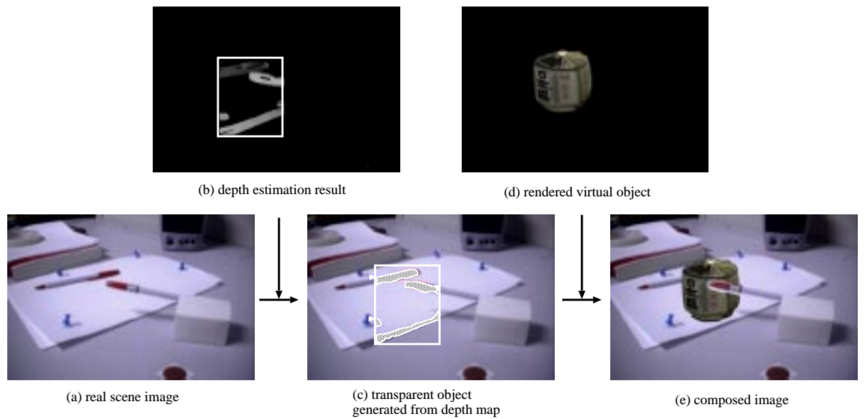
\includegraphics[width=1.0\textwidth]{content/images/methods/stereo-depth-map.png} 
  \caption{Visualisierung des Methode zur Vedeckung durch Depth Maps. Übernommen von \citet{kanbara2000stereoscopic}}
  \label{fig:stereo-depth-map}
\end{figure}

Als Erstes werden in diesem Verfahren 2D Bounding Boxen der zu rendernden virtuellen Objekte auf dem Viewport aus beiden Sichtfeldern der Stereokamera bestimmt. Die 2D Bounding Box wird durch eine Viewport Projektion der 3D Bounding Box eines virtuellen Objektes erzeugt. Diese Bounding Box Regionen wurden zunächst ermittelt, um die Bestimmung von Tiefeninformationen aus Performancegründen auf diese Bereiche zu beschränken. Als nächstes wird in den ermittelten Regionen ein Stereomatching mit Ecken aus der Anwendung des Sobel Filter durchgeführt. Hieraus können darauf folgend Tiefeninformationen der reellen Umgebung gewonnen werden. \citep{kanbara2000stereoscopic} \\

Da die Projekt Tango Hardware direkt Tiefeninformationen durch den Infrarot Laser liefert, wird das Stereomatching hier nicht weiter erläutert. Die Bestimmung von Bounding Boxen, wie von \citet{kanbara2000stereoscopic} beschrieben, ist somit auch nicht für die weitere Anwendung mit Project Tango relevant.\\

Um den Ausschluss der Pixel eines virtuellen Objektes, welches sich hinter einem reellen Objekt befinden, zu verhindern, wird der Z-Buffer Algorithmus nach \citet{greene1993hierarchical} angewendet. Dabei werden zunächst die ermittelten realen Tiefeninformationen in den Z-Buffer gefüllt. Das führt dazu, dass ein virtueller Bildpunkt des zu rendernden Objektes, welcher einen höheren Z-Wert als der bereits vorhandene Wert im Z-Buffer hat, also weiter vom Betrachter entfernt ist, nicht in den Framebuffer gelangt. In Abbildung \ref{fig:stereo-depth-map} ist das Vorgehen dieses Verfahrens noch einmal dargestellt, wobei im Fall von Project Tango Schritt \(b ) \) nicht angewendet wird. \\


